% appendixd.tex
% This work is licensed under the Creative Commons Attribution-Noncommercial-Share Alike 3.0 New Zealand License.
% To view a copy of this license, visit http://creativecommons.org/licenses/by-nc-sa/3.0/nz
% or send a letter to Creative Commons, 171 Second Street, Suite 300, San Francisco, California, 94105, USA.


\chapter{Soluções do ``Coisas para tentar''}\label{app:answers}

Aqui estão algumas respostas, para as questões das seções ``Coisas para tentar'' de cada capítulo.

\subsection*{Capítulo \ref{ch:8multipliedby3.57}}

1. A resposta para o \textbf{Exercício 1}, poderia ser algo como:

\begin{listing}
\begin{verbatim}
>>> brinquedos = ['carrinho', 'Nintendo Wii', 'computador', 'bicicleta']
>>> comidas = ['panquecas', 'chocolate', 'sorvete']
>>> favoritos = brinquedos + comidas
>>> print(favoritos)
['carrrinho', 'Nintendo Wii', 'computador', 'bicicleta', 'panquecas', 'chocolate', 'sorvete']
\end{verbatim}
\end{listing}

\noindent
2. A resposta para o \textbf{Exercício 2} é simplesmente adicionar o resultado da multiplicação de 3 por 25 e o resultado da multiplicação de 10 por 32. As seguintes equações demonstram o resultado:

\begin{listing}
\begin{verbatim}
>>> print(3 * 25 + 10 * 32)
395
\end{verbatim}
\end{listing}

\noindent
Porém, visto que vimos o uso dos parênteses no Capítulo 2, você pode ter decidido que precisa usar parênteses em algumas partes da equação. Você teria que fazer algo assim:

\begin{listing}
\begin{verbatim}
>>> print((3 * 25) + (10 * 32))
395
\end{verbatim}
\end{listing}

\noindent
A resposta é a mesma, pois a multiplicação é feita antes da adição. Nas duas equações, as duas operações de multiplicação são feitas primeiro, e os resultados são somados. Porém, a segunda equação é possivelmente um pouco melhor que a primeira --- pois, ao leitor, é imediatamente óbvio quais operações são executadas primeiro. Um programador menos experiente (que não sabe exatamente a ordem das operações) pode pensar que, na primeira equação, você multiplica 3 por 25 e adiciona 10, então multiplica o resultado por 32 (a resposta para isso é 2720 -- completamente incorreta). Com parênteses, fica mais óbvio o que é executado primeiro.

\noindent
3. A resposta para o \textbf{Exercício 3} será algo assim:

\begin{listing}
\begin{verbatim}
>>> nome = 'Maria'
>>> sobrenome = 'Almeida'
>>> print('Meu nome é %s %s' % (nome, sobrenome))
Meu nome é Maria Almeida
\end{verbatim}
\end{listing}

\subsection*{Capítulo \ref{ch:turtles}}

\noindent
1. Um retângulo é como um quadrado, exceto que dois dos seus lados são maiores que os outros dois. Dizendo à tartaruga para fazer as seguintes operações, você desenhará um retângulo:

\begin{itemize}
 \item vá um certo número de pixels à frente
 \item vire para a esquerda
 \item vá mais um pouco à frente
 \item vire para esquerda
 \item vá em frente, o mesmo número de pixels do primeiro comando
 \item vire a esquerda
 \item vá em frente, o mesmo número de pixels do segundo comando
\end{itemize}

\noindent
Por exemplo, o código seguinte desenhará o retângulo da figura\ref{fig46}.

\begin{listing}
\begin{verbatim}
>>> import turtle
>>> t = turtle.Pen()
>>> t.forward(150)
>>> t.left(90)
>>> t.forward(50)
>>> t.left(90)
>>> t.forward(150)
>>> t.left(90)
>>> t.forward(50)
\end{verbatim}
\end{listing}

\begin{figure}
\begin{center}
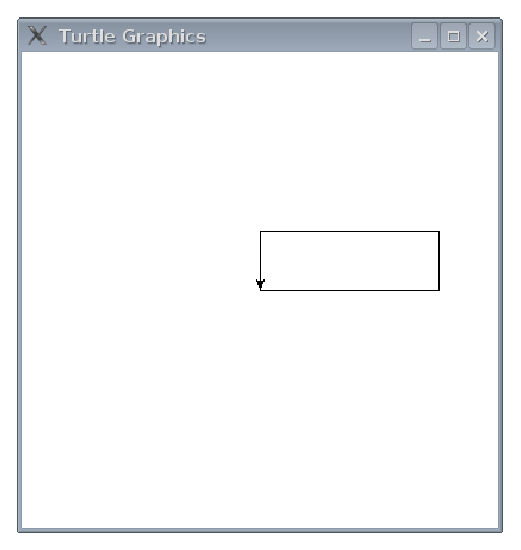
\includegraphics[width=82mm]{eps/figure46.eps}
\end{center}
\caption{A tartaruga desenhando um retângulo.}\label{fig46}
\end{figure}

\noindent
2. Um triângulo é um pouco mais complicado de desenhar, pois você precisa conhecer um pouco mais sobre ângulos e tamanho de linhas. Se você ainda não estudou ângulos na escola, então isso pode ser um pouco mais difícil do que você espera. Você pode desenhar um triângulo básico (veja na figura~\ref{fig47}), usando o seguinte código:

\begin{listing}
\begin{verbatim}
>>> import turtle
>>> t = turtle.Pen()
>>> t.forward(100)
>>> t.left(135)
>>> t.forward(70)
>>> t.left(90)
>>> t.forward(70)
\end{verbatim}
\end{listing}

\begin{figure}
\begin{center}
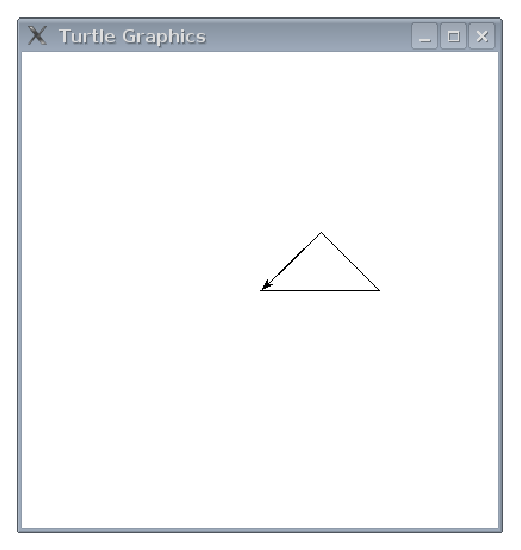
\includegraphics[width=82mm]{eps/figure47.eps}
\end{center}
\caption{A tartaruga desenhando um triângulo.}\label{fig47}
\end{figure}


\subsection*{Capítulo \ref{ch:againandagain}}

\noindent
1. O laço para após a primeira impressão. Então quando você executar oc ódigo no terminal do Python, você terá :

\begin{listing}
\begin{verbatim}
>>> for x in range(0, 20):
...     print('olá %s' % x)
...     if x < 9:
...         break
olá 0
\end{verbatim}
\end{listing}

\noindent
O motivo pelo qual ele para após o primeiro `print', é que durante a primeira execução do laço, o valor da variável \code{x} é zero. Sendo o zero menor que nove, então o comando `break' para a execução do laço imediatamente.

\noindent
2. Para descobrir quanto de dinheiro você teria quando recebesse um juros de 3\%, você precisa multiplicar o número por 0.03. Para começar, nós criamos uma variável e apontamos à ela o valor das nossas economias:

\begin{listing}
\begin{verbatim}
>>> total = 100
\end{verbatim}
\end{listing}

O total de juros recebidos ao decorrer de 1 ano, será o total multiplicado por 0.03:

\begin{listing}
\begin{verbatim}
>>> total = 100
>>> print(total * 0.03)
3.0
\end{verbatim}
\end{listing}

Isso seria R\$3! Nada mal, desde que não precisemos fazer nada para conseguí-lo. Nós precisamos imprimir esse valor e adicioná-lo ao total, e fazer isso por 10 vezes para chegar aos juros uqe vamos conseguir em 10 anos:

\begin{listing}
\begin{verbatim}
>>> total = 100
>>> for ano in range(1, 11):
...     rendimento = total * 0.03
...     print('o rendimento no ano %s é de %s' % (ano, rendimento))
...     total = total + rendimento
... 
o rendimento no ano 1 é de 3.0
o rendimento no ano 2 é de 3.09
o rendimento no ano 3 é de 3.1827
o rendimento no ano 4 é de 3.278181
o rendimento no ano 5 é de 3.37652643
o rendimento no ano 6 é de 3.4778222229
o rendimento no ano 7 é de 3.58215688959
o rendimento no ano 8 é de 3.68962159627
o rendimento no ano 9 é de 3.80031024416
o rendimento no ano 10 é de 3.91431955149
\end{verbatim}
\end{listing}

Na primeira linha, nós criamos um laço `for' usando a variável \code{year} e a função \code{range}, para contar de 1 à 10. A segunda linha, calcula o rendimento, multiplicando o valor da variável \code{total} por 0.03. Na próxima linha, está o comando `print' --- que imprime os valores do \code{ano} e \code{rendimento}. Finalmente, na última linha, nós adicionamos o rendimento de volta ao total.
Todas as casas decimais --- os números após o ponto (.), nas linhas de `print' --- confudem um pouco, mas você pode que o total do rendimento após cada ano, cresce um pouco confome você adiciona o rendimento.
O código pode ficar um pouco mais útil, se adicionarmos o total ganho a cada ano:

\begin{listing}
\begin{verbatim}
>>> total = 100
>>> for ano in range(1, 11):
...     rendimento = total * 0.03
...     print('rendimento por economizar %s em %s é %s' % 
...         (total, ano, rendimento))
...     total = total + rendimento
... 
rendimento por economizar 100 em 1 é 3.0
rendimento por economizar 103.0 em 2 é 3.09
rendimento por economizar 106.09 em 3 é 3.1827
rendimento por economizar 109.2727 em 4 é 3.278181
rendimento por economizar 112.550881 em 5 é 3.37652643
rendimento por economizar 115.92740743 em 6 é 3.4778222229
rendimento por economizar 119.405229653 em 7 é 3.58215688959
rendimento por economizar 122.987386542 em 8 é 3.68962159627
rendimento por economizar 126.677008139 em 9 é 3.80031024416
rendimento por economizar 130.477318383 em 10 é 3.91431955149
\end{verbatim}
\end{listing}

\subsection*{Capítulo \ref{ch:sortoflikerecycling}}

\noindent
1. Tornando o laço `for' em uma função é fácil. A função ficaria mais ou menos assim:

\begin{listing}
\begin{verbatim}
>>> def calcular_rendimento(total, taxa):
...     for ano in range(1, 11):
...         rendimento = total * taxa
...         print('rendimento por economizar %s em %s é %s' % 
...             (total, ano, rendimento))
...         total = total + rendimento
\end{verbatim}
\end{listing}

Se você comparar a função com o código acima, você notará que além da primeira linha, existe apenas uma diferença do código original (0.03 é passado como parâmetro \code{taxa}). Pelo \code{amount} já ser uma variável, não existe a necessidade de alterar quando é passado por parâmetro. Você verá que a saída é a mesma quando você executa a função:

\begin{listing}
\begin{verbatim}
>>> calcular_rendimento(100, 0.03)
rendimento por economizar 100 em 1 é 3.0
rendimento por economizar 103.0 em 2 é 3.09
rendimento por economizar 106.09 em 3 é 3.1827
rendimento por economizar 109.2727 em 4 é 3.278181
rendimento por economizar 112.550881 em 5 é 3.37652643
rendimento por economizar 115.92740743 em 6 é 3.4778222229
rendimento por economizar 119.405229653 em 7 é 3.58215688959
rendimento por economizar 122.987386542 em 8 é 3.68962159627
rendimento por economizar 126.677008139 em 9 é 3.80031024416
rendimento por economizar 130.477318383 em 10 é 3.91431955149
\end{verbatim}
\end{listing}

\noindent
2. Alterando a função para aceitar a quantidade de anos como parâmetro, envolve pequenas mudanças:

\begin{listing}
\begin{verbatim}
>>> def calcular_rendimento(total, taxa, anos):
...     for ano in range(1, anos):
...         rendimento = total * taxa
...         print('rendimento por economizar %s em %s é %s' %
...             (total, ano, rendimento))
...         total = total + rendimento
\end{verbatim}
\end{listing}

\noindent
Nós podemos agora, facilmente alterar o total, a taxa de rendimento e o número de anos:

\begin{listing}
\begin{verbatim}
>>> calcular_rendimento(1000, 0.05, 6)
rendimento por economizar 1000 em 1 é 50.0
rendimento por economizar 1050.0 em 2 é 52.5
rendimento por economizar 1102.5 em 3 é 55.125
rendimento por economizar 1157.625 em 4 é 57.88125
rendimento por economizar 1215.50625 em 5 é 60.7753125
\end{verbatim}
\end{listing}

\noindent
3. Um mini-programa é um pouco mais complicado do que as funções que nós já fizemos. Primeiramente, nós precisamos importar o módulo `sys' para pedirmos alguns dados. Então nós precisamos pedir ao usuário do programa, cada um dos dados. Fora isso, a função será a mesma:

\begin{listing}
\begin{verbatim}
>>> import sys
>>> def calcular_rendimento():
...     print('Digite o total que você quer guardar')
...     total = float(sys.stdin.readline())
...     print('Digite a taxa de juros')
...     taxa = float(sys.stdin.readline())
...     print('Digite o número de anos')
...     anos = int(sys.stdin.readline())
...     for ano in range(1, anos):
...         rendimento = total * taxa
...         print('rendimento por economizar %s em %s é %s' % 
...             (total, taxa, rendimento))
...         total = total + rendimento
\end{verbatim}
\end{listing}

\noindent
Quanto nós rodarmos a função, nós veremos algo parecido com o seguinte:

\begin{listingignore}
\begin{verbatim}
>>> calcular_rendimento()
Digite o total que você quer guardar
500
Digite a taxa de juros
0.06
Digite o número de anos
12
rendimento por economizar 500.0 em 1 é 30.0
rendimento por economizar 530.0 em 2 é 31.8
rendimento por economizar 561.8 em 3 é 33.708
rendimento por economizar 595.508 em 4 é 35.73048
rendimento por economizar 631.23848 em 5 é 37.8743088
rendimento por economizar 669.1127888 em 6 é 40.146767328
rendimento por economizar 709.259556128 em 7 é 42.5555733677
rendimento por economizar 751.815129496 em 8 é 45.1089077697
rendimento por economizar 796.924037265 em 9 é 47.8154422359
rendimento por economizar 844.739479501 em 10 é 50.6843687701
rendimento por economizar 895.423848271 em 11 é 53.7254308963
\end{verbatim}
\end{listingignore}

\subsection*{Capítulo \ref{ch:turtlesgalore}}

\noindent
1. Existe uma forma difícil e uma fácil de desenhar um octágo. A forma difícil não é difícil por ser complicada, é difícil pois requer muita digitação:

\begin{listing}
\begin{verbatim}
import turtle
t = turtle.Pen()
>>> t.forward(50)
>>> t.right(45)
>>> t.forward(50)
>>> t.right(45)
>>> t.forward(50)
>>> t.right(45)
>>> t.forward(50)
>>> t.right(45)
>>> t.forward(50)
>>> t.right(45)
>>> t.forward(50)
>>> t.right(45)
>>> t.forward(50)
>>> t.right(45)
>>> t.forward(50)
\end{verbatim}
\end{listing}

\noindent
You can see from that code that we tell the turtle to move forward 50 pixels, then turn right 45 degrees.  We do this 8 times.  Which is a lot of time.  The easier way to draw an octagon is the following code (which produces the octagon in figure~\ref{fig48}):

\begin{listing}
\begin{verbatim}
>>> for x in range(0,8):
...     t.forward(50)
...     t.right(45)
\end{verbatim}
\end{listing}

\begin{figure}
\begin{center}
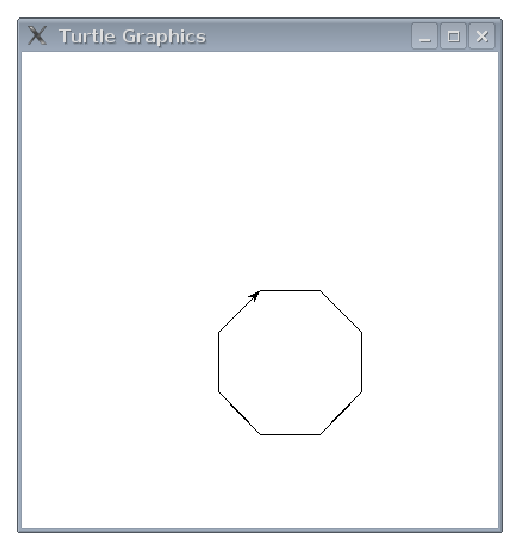
\includegraphics[width=82mm]{eps/figure48.eps}
\end{center}
\caption{Turtle drawing an octagon.}\label{fig48}
\end{figure}

\noindent
2.  If you take another look at the other functions in Chapter~\ref{ch:turtlesgalore}, you'll already see how to create a filled shape. We can convert the octagon code into a function that takes a colour, but we'll also want to reuse the hexcolour function 

\begin{listing}
\begin{verbatim}
>>> def octagon(red, green, blue):
...     t.color(red, green, blue)
...     t.begin_fill()
...     for x in range(0,8):
...         t.forward(50)
...         t.right(45)
...     t.end_fill()
\end{verbatim}
\end{listing}

We set the colour, then turn filling on.  Then we run the for loop to draw the octagon, finally we switch filling back off again to fill in the shape. How about a blue octagon (see figure~\ref{fig49}):

\begin{listing}
\begin{verbatim}
>>> octagon(0, 0, 1)
\end{verbatim}
\end{listing}

\begin{figure}
\begin{center}
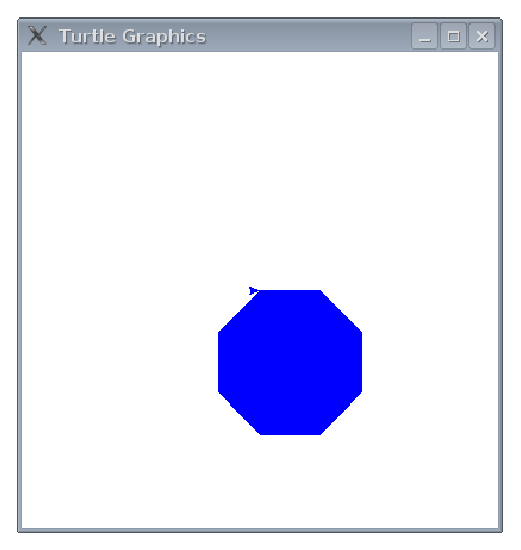
\includegraphics[width=82mm]{eps/figure49.eps}
\end{center}
\caption{Turtle drawing a blue octagon.}\label{fig49}
\end{figure}
\newpage
